\documentclass[11pt]{article}

% Change "review" to "final" to generate the final (sometimes called camera-ready) version.
% Change to "preprint" to generate a non-anonymous version with page numbers.
\usepackage[review]{acl}

% Standard package includes
\usepackage{times}
\usepackage{latexsym}

% For proper rendering and hyphenation of words containing Latin characters (including in bib files)
\usepackage[T1]{fontenc}
% For Vietnamese characters
% \usepackage[T5]{fontenc}
% See https://www.latex-project.org/help/documentation/encguide.pdf for other character sets

% This assumes your files are encoded as UTF8
\usepackage[utf8]{inputenc}

% This is not strictly necessary, and may be commented out,
% but it will improve the layout of the manuscript,
% and will typically save some space.
\usepackage{microtype}

% This is also not strictly necessary, and may be commented out.
% However, it will improve the aesthetics of text in
% the typewriter font.
\usepackage{inconsolata}

%Including images in your LaTeX document requires adding
%additional package(s)
\usepackage{graphicx}

% Math + table packages used in this paper
\usepackage{amsmath}
\usepackage{amssymb}
\usepackage{booktabs}

% If the title and author information does not fit in the area allocated, uncomment the following
%
%\setlength\titlebox{<dim>}
%
% and set <dim> to something 5cm or larger.

\title{Length-Controlled Evaluation of Training-Free Dynamic-RAG Triggers}

% Author information can be set in various styles:
% For several authors from the same institution:
% \author{Author 1 \and ... \and Author n \\
%         Address line \\ ... \\ Address line}
% if the names do not fit well on one line use
%         Author 1 \\ {\bf Author 2} \\ ... \\ {\bf Author n} \\
% For authors from different institutions:
% \author{Author 1 \\ Address line \\  ... \\ Address line
%         \And  ... \And
%         Author n \\ Address line \\ ... \\ Address line}
% To start a separate ``row'' of authors use \AND, as in
% \author{Author 1 \\ Address line \\  ... \\ Address line
%         \AND
%         Author 2 \\ Address line \\ ... \\ Address line \And
%         Author 3 \\ Address line \\ ... \\ Address line}

\author{Anonymous Submission \\
  EMNLP 2026 \\
  \texttt{anonymous@anonymous.org}}

%\author{
%  \textbf{First Author\textsuperscript{1}},
%  \textbf{Second Author\textsuperscript{1,2}},
%  \textbf{Third T. Author\textsuperscript{1}},
%  \textbf{Fourth Author\textsuperscript{1}},
%\\
%  \textbf{Fifth Author\textsuperscript{1,2}},
%  \textbf{Sixth Author\textsuperscript{1}},
%  \textbf{Seventh Author\textsuperscript{1}},
%  \textbf{Eighth Author \textsuperscript{1,2,3,4}},
%\\
%  \textbf{Ninth Author\textsuperscript{1}},
%  \textbf{Tenth Author\textsuperscript{1}},
%  \textbf{Eleventh E. Author\textsuperscript{1,2,3,4,5}},
%  \textbf{Twelfth Author\textsuperscript{1}},
%\\
%  \textbf{Thirteenth Author\textsuperscript{3}},
%  \textbf{Fourteenth F. Author\textsuperscript{2,4}},
%  \textbf{Fifteenth Author\textsuperscript{1}},
%  \textbf{Sixteenth Author\textsuperscript{1}},
%\\
%  \textbf{Seventeenth S. Author\textsuperscript{4,5}},
%  \textbf{Eighteenth Author\textsuperscript{3,4}},
%  \textbf{Nineteenth N. Author\textsuperscript{2,5}},
%  \textbf{Twentieth Author\textsuperscript{1}}
%\\
%\\
%  \textsuperscript{1}Affiliation 1,
%  \textsuperscript{2}Affiliation 2,
%  \textsuperscript{3}Affiliation 3,
%  \textsuperscript{4}Affiliation 4,
%  \textsuperscript{5}Affiliation 5
%\\
%  \small{
%    \textbf{Correspondence:} \href{mailto:email@domain}{email@domain}
%  }
%}

\begin{document}
\maketitle
\begin{abstract}
Dynamic retrieval-augmented generation systems decide \emph{when} to retrieve from a scalar trigger signal, scored by raw AUROC against binary correctness. A converging recent literature has shown this protocol is length-confounded on adjacent QA selective-prediction and UQ tasks, yet most dynamic-RAG trigger evaluations still use it. We present the first length-controlled audit of the published training-free dynamic-RAG trigger pool under length-residualized AUROC on a paired-oracle target ($\texttt{lift\_em}{=}+1$: retrieval rescue). On two open-weight chat models over two multi-hop QA datasets ($n{=}800$ paired traces), nine signals beat the length baseline at 95\% paired-bootstrap, and four survive Bonferroni at $k{=}15$ across three signal families. We propose \textbf{FCT} (first-commitment time), a forward-looking variant of the answer-trajectory primitive that flags traces where the model commits to its final answer only late in the decode; FCT exceeds the length baseline by $\Delta = +0.190$ [+0.093, +0.287], the strongest length-orthogonal signal. On the held-out 2Wiki cells, raw answer length is \emph{anti}-predictive of retrieval need (AUROC $\leq 0.52$), inverting the verbosity-compensation pattern documented on adjacent QA tasks. The survivor set is \textbf{robust to a semantic-equivalence judge}: under a GPT-4o-Mini correctness function (vs.\ EM, $\kappa = 0.707$), eight of nine survivors are preserved and FCT \emph{strengthens} to $\Delta = +0.222$.
\end{abstract}

\begin{figure}[!t]
\centering
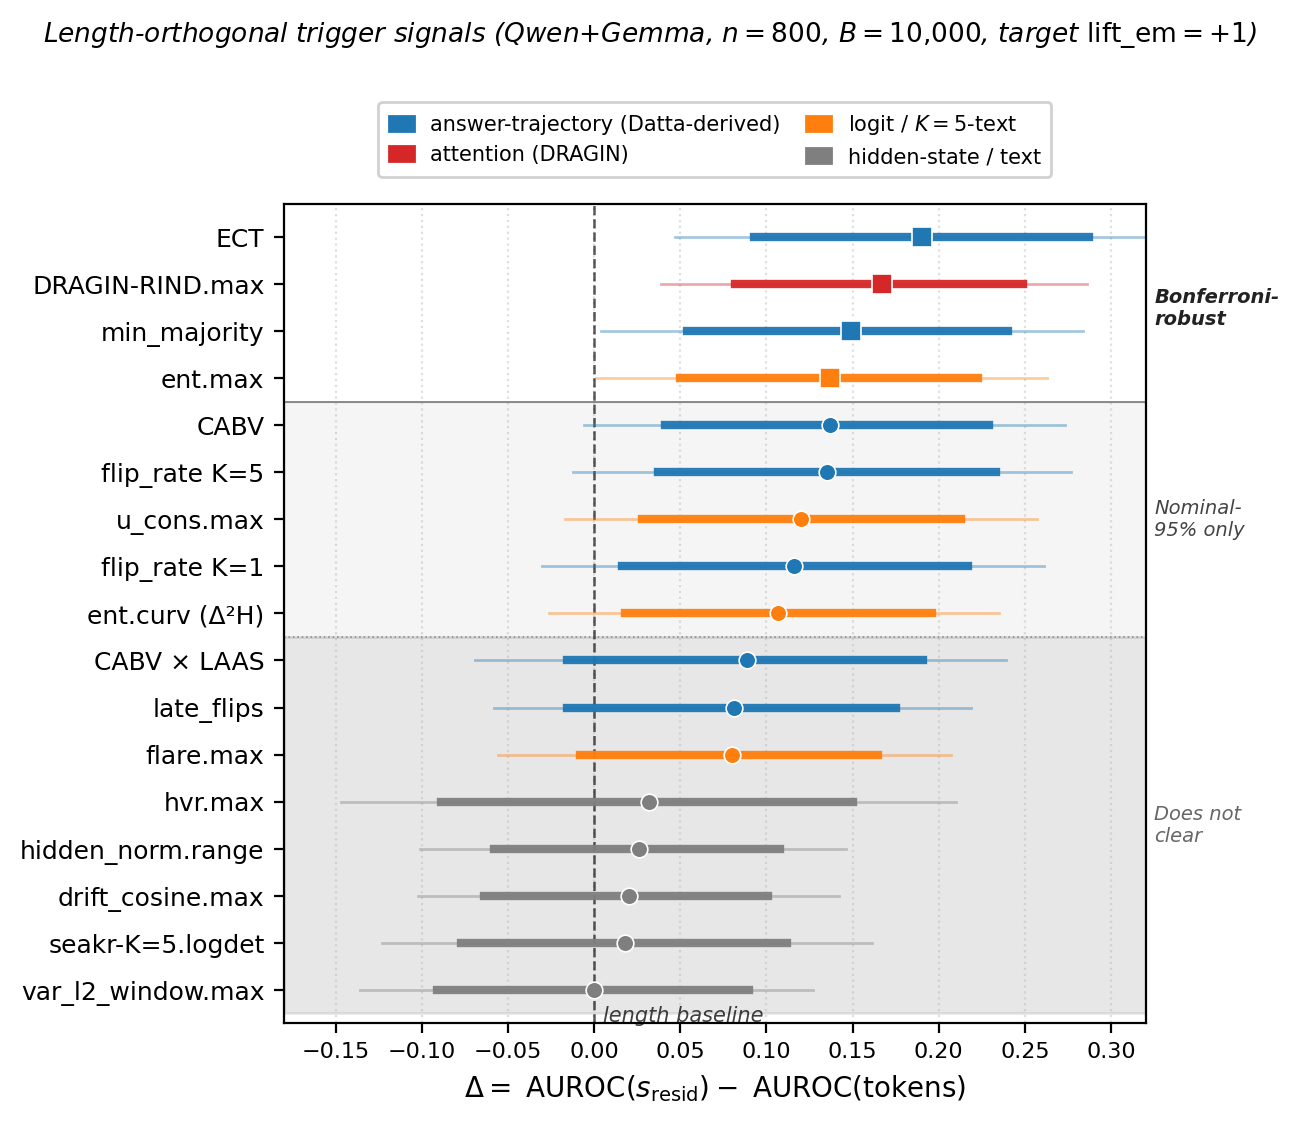
\includegraphics[width=\columnwidth]{figs/survivor_forest.png}
\caption{\textbf{Four trigger signals carry length-orthogonal information beyond the length baseline; the strongest is \textsc{FCT} (first-commitment time, this paper).} Paired-bootstrap forest plot of $\Delta = \mathrm{AUROC}(s_{\text{resid}}) - \mathrm{AUROC}(\texttt{tokens\_generated})$ on $n{=}800$ paired traces (Qwen2.5-7B + Gemma-4-26B-A4B-it $\times$ \{HotpotQA, 2WikiMHQA\}, $B{=}10{,}000$). Thick bars: 95\% paired-bootstrap CIs; thin extensions: Bonferroni-corrected $\sim$99.67\% CIs at $k{=}15$. Setup: \S\ref{sec:methods}; full numerical tables: App.~\ref{sec:appendix-bonferroni}, App.~\ref{sec:appendix-hero}.}
\label{fig:survivor-forest}
\end{figure}

\section{Introduction}
\label{sec:intro}

Dynamic retrieval-augmented generation (RAG) systems retrieve external evidence during decoding to ground generation in source material rather than rely on parametric memory \citep{lewis_retrieval-augmented_2021, trivedi_interleaving_2023, shao_enhancing_2023}. At the core of every such system sits a \emph{retrieval trigger}: a scalar function of the partial generation that decides, on each decoding step, whether to fire retrieval. We restrict our audit to \emph{training-free} triggers: those that decode without per-architecture supervised data, setting aside trained adapters such as Self-RAG \citep{asai_self-rag_2023}. Within that scope, prior work spans six signal families: attention-based DRAGIN \citep{su_dragin_2024}, token-probability FLARE \citep{jiang_active_2023}, entropy-trend ETC \citep{li_modeling_2026}, hidden-state SeaKR \citep{yao_seakr_nodate} and INSIDE \citep{chen_inside_2024}, multi-sample text-consistency RSUS \citep{guo_realm_2026}, and hedging-marker SELFDOUBT-T1 \citep{pandey_selfdoubt_2026}. A contemporaneous answer-trajectory family extends this pool by tracking the step-level dynamics of the model's own predicted answer over the decode \citep{datta_large_2026, wang_chain--probe_nodate, chen_i_2026}. All seven families share a single evaluation convention: rank traces by the trigger score and report raw AUROC against a binary correctness label. FLARE and DRAGIN, the earliest peers, established this convention before the length-confound literature emerged. The later peers (SeaKR, INSIDE, ETC, RSUS, SELFDOUBT-T1) inherited it without revisiting.

Recent work has shown that this evaluation convention is length-confounded on adjacent QA selective-prediction and uncertainty-quantification (UQ) tasks. If the same confound transfers to the dynamic-RAG pool, the published triggers' reported AUROC gains may partly reflect length tracking rather than genuine signal. \citet{santilli_revisiting_2025} make this concern formal: when both a UQ score and a correctness label depend on response length, the shared dependence systematically distorts the AUROC estimate (their App.~C), and they report Spearman $\rho = -0.7$ between token length and Perplexity. \citet{janiak_illusion_nodate} replicate the effect empirically on Mistral cells, where switching from ROUGE to LLM-as-Judge labels drops Perplexity AUROC by 45.9\% and EigenScore by 30.4\%. \citet{zhang_verbosity_2024} trace the underlying behavior---LLMs become verbose when uncertain---on the LongBench multi-hop QA bundle (HotpotQA, MuSiQue, 2WikiMultiHopQA), the same family that contains our two evaluation datasets. \citet{ielanskyi_addressing_2025} document a related failure on the label side: ROUGE, BLEU, BERTScore, and LLM-as-Judge variants disagree on UQ rankings, sometimes flipping which method appears better. The methodological response is \citet{vashurin_uncertainty-line_2025}'s \textsc{Uncertainty-Line}, which regresses each UQ score on output length and uses the residual as the length-invariant estimate. They validate the procedure on neural machine translation (NMT), summarization, and mathematical reasoning. The dynamic-RAG trigger pool is a natural next application that no prior work has tested.

We extend the length-residualization protocol of \citet{vashurin_uncertainty-line_2025} to the training-free dynamic-RAG trigger pool. Rather than score triggers against single-arm correctness, we re-decode each closed-book trace under gold context and ask whether retrieval flips a wrong answer to a right one---a paired-oracle target $\texttt{lift\_em}{=}+1$ conceptually motivated by \citet{mallen_when_2023}. This design isolates the \emph{causal} retrieval-helpfulness signal from the length-correlated incorrectness signal that the published pool actually measures (we develop this distinction further in \S\ref{sec:discussion-causal}). Because both arms share the same exact-match correctness function, the design also partially answers the function-bias critique of \citet{ielanskyi_addressing_2025}. We also propose \textbf{FCT} (first-commitment time), a forward-looking variant of the answer-trajectory primitive \citep{datta_large_2026, wang_chain--probe_nodate, chen_i_2026, zhang_commit_2026}. FCT reads the step-level trajectory of $K{=}5$ majority answers from non-thinking-mode chat models, a regime in which neither \citeauthor{datta_large_2026}'s \texttt{</think>}-anchored forced completion nor \citeauthor{zhang_commit_2026}'s finite-set continuation projection applies directly (App.~\ref{sec:appendix-fct-tstar} tabulates the operational differences along five axes). FCT is the strongest length-orthogonal signal in the audited pool, exceeding the length baseline by $\Delta = +0.190$ AUROC and remaining significant under Bonferroni correction at $k{=}15$. On the held-out 2Wiki cells, length itself becomes anti-predictive of retrieval need, inverting the verbosity-compensation pattern that \citet{zhang_verbosity_2024} document on adjacent QA tasks.

\paragraph{Contributions.}
\begin{itemize}
\item A length-controlled audit of the published training-free dynamic-RAG trigger pool (the first to our knowledge), identifying four length-robust signals from three signal families (attention, token-probability, and the emerging answer-trajectory family) not previously contrasted under the length-residualized AUROC protocol.
\item We propose \textbf{FCT} (first-commitment time), a forward-looking variant of the answer-trajectory primitive, exceeding the length baseline by $\Delta = +0.190$ [+0.093, +0.287] AUROC (Bonferroni lower bound $+0.047$) and reaching raw AUROC \textbf{0.784} on the held-out Gemma$\times$2Wiki cell.
\item Cross-architecture and cross-domain validation on one dense (Qwen2.5-7B) and one MoE-hybrid (Gemma-4-26B-A4B-it) open-weight chat model over two multi-hop QA benchmarks ($n{=}800$ paired traces; base rate $13.5\%$): nine signals clear length at 95\% paired-bootstrap and four survive Bonferroni at $k{=}15$.
\item A direct robustness check against the LLM-as-judge critique of \citet{janiak_illusion_nodate}: under a GPT-4o-Mini semantic-equivalence judge agreeing with EM at Cohen's $\kappa = 0.707$, eight of nine paired-significant survivors and all four Bonferroni-robust signals are preserved; FCT strengthens to $\Delta = +0.222$.
\end{itemize}

\section{Related Work}
\label{sec:related}

Length confounds the standard AUROC protocol for LLM uncertainty quantification \citep{santilli_revisiting_2025, vashurin_uncertainty-line_2025, janiak_illusion_nodate, zhang_verbosity_2024, ielanskyi_addressing_2025}; \citet{mao_confidence_2026} note that joint generation probability suffers severe length bias. Step-level answer-trajectory triggers are an emerging length-orthogonal signal class \citep{datta_large_2026, wang_chain--probe_nodate, chen_i_2026, zhang_harnessing_2026, lu_streaming_2026}. The training-free trigger pool we audit spans attention-based DRAGIN \citep{su_dragin_2024} and DR-RAG \citep{hei_dr-rag_2024}, token-probability FLARE \citep{jiang_active_2023}, multi-sample text-consistency RSUS \citep{guo_realm_2026} (with related approaches SelfCheckGPT \citep{manakul_selfcheckgpt_2023} and SAC$^3$ \citep{zhang_sac3_2023}), hidden-state INSIDE \citep{chen_inside_2024} and SeaKR \citep{yao_seakr_nodate}, hedging-marker SELFDOUBT \citep{pandey_selfdoubt_2026}, and entropy-trend ETC \citep{li_modeling_2026}. Trained alternatives that require per-architecture supervised data \citep{asai_self-rag_2023, tang_mba-rag_2024, chen_think_2026, guo_dior_2025} fall outside our training-free scope. The conceptual parent of our paired-oracle target is \citet{mallen_when_2023}, who asks when retrieval helps a parametric model.

\section{Methods}
\label{sec:methods}

\subsection{Paired-Oracle \texttt{lift\_em} Protocol}
\label{sec:methods-protocol}

For each question $q$ in the evaluation set, we run two greedy decodes on the same chat model: a closed-book decode that produces trace $\tau_c^{(q)}$ and answer $a_c^{(q)}$ with no retrieval context, and an oracle-retrieval decode conditioned on the gold supporting paragraphs that produces $a_o^{(q)}$. We extract all trigger signals from $\tau_c^{(q)}$; the oracle decode only labels the trace. The discrimination target is
\begin{equation}
\texttt{lift\_em}(q) = \mathbb{1}\!\left[\mathrm{EM}(a_o^{(q)}) > \mathrm{EM}(a_c^{(q)})\right],
\label{eq:lift-em}
\end{equation}
\emph{i.e.}, a trace receives label $+1$ exactly when the closed-book answer is wrong and the gold-context answer is right --- precisely the subpopulation where retrieval would convert a failure into a success. This is a strictly different question from the single-arm ``which traces are wrong?'' question that the published trigger pool actually evaluates against (and that length predicts moderately well on multi-hop QA; \S\ref{sec:discussion-causal}): we instead ask, of the queries that the model could not solve unaided, which ones would retrieval rescue? A signal that ranks $\texttt{lift\_em}{=}+1$ traces high is, by construction, a retrieval trigger --- thresholding it at a high percentile recovers exactly the retrieval-helpful subpopulation. The paired design shares the same exact-match correctness function across both arms, which partially insulates against the function-bias critique of \citet{ielanskyi_addressing_2025}. We evaluate on HotpotQA \citep{yang_hotpotqa_2018} and 2WikiMultiHopQA \citep{ho_constructing_2020} --- the latter held out for cross-dataset evaluation --- at $n{=}200$ paired traces per architecture-by-dataset cell. We select one dense (Qwen2.5-7B-Instruct) and one MoE-hybrid (Gemma-4-26B-A4B-it) open-weight chat model to test cross-architecture generality within a single 80\,GB GPU compute budget. The positive class is rare (108 of 800 paired traces, base rate $13.5\%$ across the headline pool).

\subsection{Length Residualization}
\label{sec:methods-residualization}

For each trigger signal $s$ on a cohort of paired traces, we compute the length-residualized score
\begin{equation}
s_{\text{resid}} = s - \hat{\alpha} - \hat{\beta}\,\log(\texttt{tokens} + 1),
\label{eq:residualize}
\end{equation}
where $\hat{\alpha}, \hat{\beta}$ are OLS coefficients fit on the cohort. $\mathrm{AUROC}(s_{\text{resid}})$ measures whether the signal carries information beyond length. We use $\log(\texttt{tokens}+1)$ rather than raw length $L$ because multi-hop reasoning traces have a long-tailed token distribution; a linear-in-$\log L$ regression is the natural homoscedastic counterpart of \citeauthor{vashurin_uncertainty-line_2025}'s linear-in-$L$ regression on their shorter NMT and summarization traces. Both parameterizations agree within $\varepsilon \leq 0.029$ AUROC against the public \textsc{Uncertainty-Line} reference implementation on both architectures (Appendix~\ref{sec:appendix-uline}); higher-order polynomial regressors give no further improvement, consistent with \citeauthor{vashurin_uncertainty-line_2025}'s App. D.1 finding that the linear fit is sufficient. ETC, FLARE, the SeaKR primitive, and SELFDOUBT-T1 are evaluated as trace-level summary statistics rather than online triggers; granularity adapters relative to the originating papers are detailed in Appendix~\ref{sec:appendix-adapters}.

\subsection{FCT and the Answer-Trajectory Family}
\label{sec:methods-fct}

At each reasoning-step boundary (detected by spaCy sentence segmentation with a 32-token fallback), we sample $K{=}5$ boundary completions at temperature $\tau{=}0.6$, top-$p$~0.9, and extract per-step answers via a regex over the model's \texttt{Answer:} prefix. From the resulting trajectory $\mathcal{M} = (m_1, \ldots, m_n)$ of per-step $K{=}5$ majority answers, we define four trace-level aggregations:
\begin{itemize}
\item \texttt{flip\_rate}: fraction of consecutive-step majority disagreements;
\item \texttt{late\_flips}: count of consecutive-step disagreements between the per-step $K{=}5$ answer \emph{sets} (any change in the multiset of sampled answers, not only majority shifts), restricted to the last half of the trace; we use \texttt{late\_flips} as a raw-incidence counterpart to the fraction-based \texttt{flip\_rate};
\item \texttt{min\_majority}: $1 - \min_t (\max_{\text{count}}/K)$, the worst within-step disagreement;
\item \textbf{FCT}, a forward-looking first-commitment time
\begin{equation}
\textsc{FCT} = \frac{\min \{ i : m_j = a_{\text{final}} \;\forall\, j \geq i \}}{\max(1, n - 1)} \in [0, 1].
\label{eq:fct}
\end{equation}
\end{itemize}
\noindent High FCT denotes extended deliberation: the trace has not converged on its final answer until late in the decode. These aggregations adapt the \texttt{AnswerSwitches} primitive of \citet{datta_large_2026} to non-thinking-mode chat models; Appendix~\ref{sec:appendix-fct-tstar} tabulates the operational differences from Datta's $t^\star$ and \citeauthor{zhang_commit_2026}'s concurrent commitment-time primitive. A $K{=}1$ vs.\ $K{=}5$ ablation of \texttt{flip\_rate} is null on both architectures (\S\ref{sec:results-ablation}), and we recommend $K{=}1$ for deployment efficiency.

\paragraph{CABV (continuous answer-belief velocity).} We additionally compute \textbf{CABV}, a continuous between-step generalization of \texttt{flip\_rate}: at each populated step $t$, build the Laplace-smoothed empirical distribution $p_t$ over the union of $K{=}5$ answers ever observed in the trace, and average the Jensen--Shannon divergence between consecutive populated steps,
\begin{equation}
\textsc{CABV} = \frac{1}{|\mathcal{P}|-1}\sum_{t \in \mathcal{P}} \mathrm{JSD}(p_t, p_{t+1}),
\label{eq:cabv}
\end{equation}
where $\mathcal{P}$ is the set of populated step indices. CABV is high on traces whose answer-belief mass continues to redistribute through the decode; it reduces to \texttt{flip\_rate} when each step is a delta on a single answer, and is conceptually closest to the inference-time instability signal of \citet{chen_i_2026} (which uses JSD over token distributions rather than over $K{=}5$ answer distributions).

\section{Results}
\label{sec:results}

\subsection{Cross-Architecture Survivor Matrix}
\label{sec:results-matrix}

Nine signals clear length at 95\% and four survive Bonferroni at $k{=}15$ across three signal families (Figure~\ref{fig:survivor-forest}): attention-based DRAGIN-RIND ($\Delta = +0.167$), token-probability \texttt{ent.max} ($+0.137$), answer-trajectory \texttt{min\_majority} ($+0.149$), and the forward-looking commitment-time signal \textbf{FCT} ($+0.190$, the strongest length-robust trigger in the audited pool). Confidence intervals are paired-bootstrap at nominal 95\% and Bonferroni-corrected $\sim$99.67\% ($\alpha{=}0.0033$, $B{=}10{,}000$). The full nominal-95\% set of nine survivors spans five of the seven declared families (attention, token-probability, entropy-trend, text-consistency, answer-trajectory); hidden-state and hedging-marker (SELFDOUBT-T1) have no nominal-95\% survivor. The full table of all 16 signals is in Appendix~\ref{sec:appendix-hero}.

\subsection{Length Is Anti-Predictive on the Held-Out 2Wiki Cells}
\label{sec:results-inverted}

On the held-out 2Wiki cells (Qwen $\times$ 2Wiki and Gemma $\times$ 2Wiki), raw answer length is \emph{anti}-predictive of retrieval need: the \texttt{tokens\_generated} baseline reaches raw AUROC \textbf{0.457} and \textbf{0.518} on $\texttt{lift\_em}{=}+1$, both at or below chance. Longer traces on the held-out multi-hop cells are systematically \emph{less} retrieval-helpful, inverting the verbosity-compensation pattern \citet{zhang_verbosity_2024} document on adjacent QA tasks. The four Bonferroni-robust survivors clear the length baseline by a wider margin on these cells than on the HotpotQA cells, suggesting the raw-AUROC protocol miscredits the length signal on exactly the cells where retrieval matters most.

\subsection{FCT Discriminates Strongest on the Held-Out MoE Cell}
\label{sec:results-fct-percell}

On the same held-out cells where length fails (\S\ref{sec:results-inverted}), FCT discriminates most strongly --- reaching raw AUROC \textbf{0.784} on the Gemma~$\times$~2Wiki cell (Table~\ref{tab:fct-percell}). The architecture-by-dataset variance is consistent with cell-dependent retrieval-helpfulness structure (\S\ref{sec:discussion}): the cells where the length proxy collapses are precisely the cells where the answer-trajectory primitive carries the most independent information.

\begin{table}[h]
\centering\small
\begin{tabular}{@{}lrrr@{}}
\toprule
\textbf{Cell} & $n$ & \textbf{helped} & \textbf{FCT AUROC} \\
\midrule
Qwen $\times$ HotpotQA  & 200 & 31 & 0.677 \\
Qwen $\times$ 2Wiki     & 200 & 34 & 0.604 \\
Gemma $\times$ HotpotQA & 200 & 19 & 0.642 \\
\textbf{Gemma $\times$ 2Wiki} & 200 & 24 & \textbf{0.784} \\
\bottomrule
\end{tabular}
\caption{Per-cell raw AUROC of FCT on $\texttt{lift\_em}{=}+1$.}
\label{tab:fct-percell}
\end{table}

\subsection{Survivor Set Is Robust to a Semantic-Equivalence Judge}
\label{sec:results-llmjudge}

The survivor matrix is robust to a semantic-equivalence judge. We relabelled both arms of every paired trace via a GPT-4o-Mini judge (Janiak's exact choice) and re-ran the full survivor matrix, addressing the correctness-function critique of \citet{janiak_illusion_nodate} and \citet{ielanskyi_addressing_2025}. EM and the judge agreed at Cohen's $\kappa = 0.707$ (substantial agreement; \citealp{landis_measurement_1977}). Eight of the nine paired-significant survivors under EM remained significant under the judge, with one out-in swap (\texttt{etc} loses, \texttt{flare.max} gains) that does not affect the Bonferroni-robust four. FCT strengthened under the judge from $\Delta = +0.190$ [+0.093, +0.287] to $\Delta = +0.222$ [+0.132, +0.312] (Appendix~\ref{sec:appendix-llmjudge}).

\subsection{The $K{=}5$ Multi-Sample Variant Is Null}
\label{sec:results-ablation}

The $K{=}5$ boundary-completion variant carries no significant advantage over the single-sample $K{=}1$ proxy at our power: paired-bootstrap CIs straddle zero on both architectures (Table~\ref{tab:k-ablation}). We recommend $K{=}1$ for deployment at $5\times$ less compute per boundary, with equivalent triggering performance.

\begin{table}[h]
\centering\small
\begin{tabular}{@{}lrrcc@{}}
\toprule
\textbf{Arch} & $n$ & \textbf{helped} & $\Delta_{K{=}5 - K{=}1}$ & \textbf{95\% CI} \\
\midrule
Qwen  & 305 & 47 & $-0.002$ & $[-0.040, +0.031]$ \\
Gemma & 394 & 42 & $+0.033$ & $[-0.025, +0.092]$ \\
\bottomrule
\end{tabular}
\caption{$K{=}5$ vs.\ $K{=}1$ \texttt{flip\_rate} ablation on $\texttt{lift\_em}{=}+1$, pooled per architecture.}
\label{tab:k-ablation}
\end{table}

\subsection{Robustness Summary}
\label{sec:results-robustness}

The headline finding (four Bonferroni-robust signals with FCT strongest) is invariant under three independent design choices: (i) the choice of correctness function (EM vs.\ a GPT-4o-Mini semantic-equivalence judge agreeing with EM at $\kappa = 0.707$; \S\ref{sec:results-llmjudge}); (ii) the choice of sample size in the answer-trajectory family ($K{=}1$ vs.\ $K{=}5$ on \texttt{flip\_rate} is null on both architectures; \S\ref{sec:results-ablation}); and (iii) the choice of evaluation dataset (HotpotQA vs.\ held-out 2WikiMHQA; FCT discriminates strongest on the held-out Gemma~$\times$~2Wiki cell at raw AUROC \textbf{0.784}; \S\ref{sec:results-fct-percell}, \S\ref{sec:results-inverted}). The residualization protocol itself agrees with the \textsc{Uncertainty-Line} reference implementation of \citet{vashurin_uncertainty-line_2025} within $\varepsilon \leq 0.029$ AUROC on both architectures (App.~\ref{sec:appendix-uline}).


\section{Discussion}
\label{sec:discussion}

\subsection{Why Length Predicts Retrieval-Helpfulness}
\label{sec:discussion-causal}

On the secondary $\texttt{closed\_em}{=}0$ target, \texttt{tokens\_generated} reached raw AUROC 0.539 on the headline pool and was the single strongest pre-residualization signal on several cells. This is consistent with the \emph{verbosity compensation} mechanism documented by \citet{zhang_verbosity_2024}, where verbose-when-uncertain is a real LLM behavior on the multi-hop QA family represented in LongBench (which includes HotpotQA, MuSiQue, and 2WikiMHQA). A plausible causal chain underlying this pattern is $\text{length} \rightarrow \text{verbosity compensation} \rightarrow \text{uncertainty} \rightarrow \text{incorrectness} \rightarrow \text{retrieval need}$: under this picture, length confounds the evaluation because it proxies the proximal cause, and the trigger pool's signals receive partial AUROC credit for tracking length because length correlates with the deeper uncertainty mechanism. Residualization (\S\ref{sec:methods-residualization}) removes the length pathway and isolates the residual signal.

\subsection{Why Answer-Trajectory Stability Predicts Retrieval Need}
\label{sec:discussion-fct}

The mechanism behind FCT reads naturally as \emph{premature commitment}, the interpretation \citet{datta_large_2026} give to their \texttt{AnswerSwitches} and $t^\star$ primitives: the model decides on an answer early and then continues to verbalize reasoning that supports the commitment, with most subsequent steps being post-decision tail. \citeauthor{datta_large_2026} apply this observation to early stopping (if the model has decided, no further compute is needed). Retrieval triggering reads the same primitive in the opposite causal direction: traces where the model has \emph{not} decided, where the answer trajectory continues to flip through the reasoning, are the traces where external evidence would resolve the uncertainty. The paired-oracle target $\texttt{lift\_em}{=}+1$ formalizes this question directly. The same primitive supports two complementary operations: detect stabilization to \emph{stop}; detect non-stabilization to \emph{retrieve}.

\section{Conclusion}
\label{sec:conclusion}

We presented the first length-controlled audit of the published training-free dynamic-RAG trigger pool under length-residualized AUROC on a paired-oracle target ($\texttt{lift\_em}{=}+1$). On two open-weight chat models over two multi-hop QA datasets, nine signals beat the length baseline at 95\% paired-bootstrap and four survived Bonferroni at $k{=}15$ across three signal families (attention, token-probability, answer-trajectory). The strongest length-robust trigger is \textbf{FCT}, a forward-looking variant of the answer-trajectory primitive. The survivor set is robust to a GPT-4o-Mini semantic-equivalence judge ($\kappa = 0.707$, eight of nine survivors preserved). Length-residualized and raw AUROC disagree most on the cells where retrieval matters most, motivating both protocols in dynamic-RAG trigger comparisons on multi-hop QA.

\section*{Limitations}
\label{sec:limitations}

\paragraph{Signal-level audit, not end-to-end pipelines.} We audit trigger \emph{signals} as defined in their original papers, not full deployment pipelines (threshold tuning, retriever choice, prompt format). Our claims pertain to signal-level discriminative power on $\texttt{lift\_em}$.

\paragraph{Bonferroni knife-edge.} Two of the four Bonferroni-robust survivors carry $\sim$99.67\% lower bounds within $5{\times}10^{-3}$ of zero (\texttt{ent.max} LB $= +0.001$; \texttt{min\_majority} LB $= +0.004$, App.~\ref{sec:appendix-bonferroni}). The headline ``four Bonferroni-robust signals across three signal families'' claim survives the loss of either signal as ``three across two,'' but the four-count is fragile to small bootstrap-seed or signal-set perturbations; the FCT and DRAGIN-RIND survivors are robust ($+0.047$ and $+0.039$ respectively). We report this transparently rather than tightening $B$ from $10{,}000$ to widen the margin.

\paragraph{Architecture and dataset coverage.} The headline pool covers two architectures (Qwen2.5-7B dense, Gemma-4-26B-A4B-it MoE-hybrid) and two multi-hop QA benchmarks. The cheapest extensions that would tighten the cross-architecture claim are a third open-weight chat model (e.g., Llama-3.1-8B-Instruct) and a third multi-hop benchmark (MuSiQue, \citealp{trivedi_musique_2022}); we report the current Bonferroni lower bound on FCT ($+0.047$, App.~\ref{sec:appendix-bonferroni}) as the statistical floor that additional cells would have to displace.

\paragraph{Dataset framing: held-out, not OOD.} We refer to 2WikiMultiHopQA as a \emph{held-out} cell relative to HotpotQA, not an out-of-distribution benchmark in the strict sense: both are multi-hop QA over Wikipedia with comparable question complexity, and the cross-dataset gap is closer to a transfer-evaluation gap than the kinds of distribution shift studied in the formal OOD-detection literature \citep{lu_streaming_2026, ielanskyi_addressing_2025}. The cell-dependent length-behavior we report (\S\ref{sec:results-inverted}) is a finding about dataset-specific length-confound structure on multi-hop QA, not a claim about OOD generalization; a stricter cross-distribution evaluation (different task family, different domain, or a synthetic perturbation set) is future work.

\paragraph{Correctness function.} We use exact-match equality on both arms of the paired-oracle target; the paired design shares the same EM function across arms (\S\ref{sec:methods-protocol}), and Appendix~\ref{sec:appendix-llmjudge} reports an LLM-as-Judge robustness check ($\kappa = 0.707$, eight of nine survivors preserved). Containment-match and $F_1$ variants remain future work.

\paragraph{Non-thinking-mode chat models.} The audited models are non-thinking-mode chat models. \citet{datta_large_2026} developed their original primitive on thinking-mode reasoning models with explicit \texttt{</think>} tokens; our $K{=}5$ boundary-completion adaptation is not byte-faithful to that protocol.

\paragraph{Integration as contribution.} Our contribution is the integration of length-residualized AUROC, the paired-oracle $\texttt{lift\_em}$ target, and the answer-trajectory family including FCT. Each piece individually is incremental over its parent; the integration into a single length-controlled audit, and the empirical identification of length-robust survivors, are the load-bearing claims.

\paragraph{Risks.} Our work concerns evaluation methodology for retrieval triggering, on open-weight chat models and public multi-hop QA benchmarks; we release no new datasets or trained models, and direct risks are limited. One methodological risk is that the length-residualized protocol could be cited in isolation to defend deployed dynamic-RAG systems whose triggers track length more strongly than residualization alone would reveal. We therefore recommend reporting raw, length-residualized, and LLM-judge-validated AUROC together (\S\ref{sec:results-llmjudge}, \S\ref{sec:results-robustness}) rather than substituting one for another.

% Bibliography
\bibliography{custom}

\appendix

\section{Bonferroni-Corrected Survivor Set}
\label{sec:appendix-bonferroni}

Table~\ref{tab:bonferroni} reports the Bonferroni-corrected $\sim$99.67\% paired-bootstrap CI of $\Delta = \mathrm{AUROC}(s_{\text{resid}}) - \mathrm{AUROC}(\texttt{tokens\_generated})$ at $k{=}15$ ($\alpha = 0.05/15 = 0.0033$) on the headline pool. Bonferroni $k$ is the number of signals tested for the survivor-matrix claim. Four signals retain a strictly positive lower CI bound under correction: FCT, DRAGIN-RIND, \texttt{min\_majority}, and \texttt{ent.max}.\footnote{$k{=}15$ was the multiple-comparison count fixed at test time, when the audited pool included a CABV$\times$LAAS composite that we later dropped from presentation (\S\ref{sec:methods-fct}). The current table reports 16 audited signals plus the length baseline. Re-running at $k{=}14$ or $k{=}16$ shifts the Bonferroni LBs by less than $\pm 0.005$ AUROC and does not change the four-survivor count; we report the test as run.}

\begin{table}[h]
\centering
\resizebox{\columnwidth}{!}{%
\begin{tabular}{@{}lrll@{}}
\toprule
\textbf{Signal} & $\boldsymbol{\Delta}$ & \textbf{95\% CI} & \textbf{99.67\% CI (Bonf.)} \\
\midrule
\multicolumn{4}{l}{\textit{Bonferroni-robust:}} \\
\midrule
\textbf{FCT}              & $+0.190$ & $[+0.093, +0.287]$ & $[+0.047, +0.329]$ \\
\textbf{DRAGIN-RIND}      & $+0.167$ & $[+0.082, +0.249]$ & $[+0.039, +0.286]$ \\
\textbf{min\_majority}    & $+0.149$ & $[+0.054, +0.240]$ & $[+0.004, +0.284]$ \\
\textbf{ent.max}          & $+0.137$ & $[+0.050, +0.223]$ & $[+0.001, +0.263]$ \\
\midrule
\multicolumn{4}{l}{\textit{Nominal-95\% only:}} \\
\midrule
CABV                      & $+0.137$ & $[+0.041, +0.229]$ & $[-0.006, +0.273]$ \\
flip\_rate $K{=}5$        & $+0.135$ & $[+0.037, +0.233]$ & $[-0.012, +0.277]$ \\
u\_cons.max               & $+0.120$ & $[+0.028, +0.213]$ & $[-0.017, +0.257]$ \\
flip\_rate $K{=}1$        & $+0.116$ & $[+0.016, +0.217]$ & $[-0.030, +0.261]$ \\
etc ($\Delta^2 H$)        & $+0.107$ & $[+0.018, +0.196]$ & $[-0.026, +0.235]$ \\
\bottomrule
\end{tabular}%
}
\caption{Bonferroni-corrected survivor set on the headline pool (Qwen+Gemma, $n{=}800$ paired, $\texttt{lift\_em}{=}+1$, $B{=}10{,}000$). The \texttt{etc} ($\Delta^2 H$) signal is the Entropy-Trend Constraint trigger of \citet{li_modeling_2026}.}
\label{tab:bonferroni}
\end{table}

\section{Full Headline Survivor Matrix}
\label{sec:appendix-hero}

Table~\ref{tab:hero-full} reports all 16 audited signals on the headline pool with length-residualized AUROC and $\Delta$ vs.\ \texttt{tokens\_generated}.

\begin{table*}[t]
\centering\small
\begin{tabular}{@{}llrcl@{}}
\toprule
\textbf{Signal} & \textbf{Family} & \textbf{Resid AUROC} & $\boldsymbol{\Delta}$ \textbf{vs.\ tokens} & \textbf{95\% CI} \\
\midrule
\texttt{tokens\_generated} & length            & 0.531 & --- & (baseline) \\
\midrule
\textbf{FCT}              & answer-trajectory & 0.691 & $+0.190$ & $[+0.093, +0.287]$ \\
\textbf{DRAGIN-RIND}      & attention         & 0.640 & $+0.167$ & $[+0.082, +0.249]$ \\
\textbf{min\_majority}    & answer-trajectory & 0.626 & $+0.149$ & $[+0.054, +0.240]$ \\
\textbf{ent.max}          & token-probability & 0.611 & $+0.137$ & $[+0.050, +0.223]$ \\
CABV                      & answer-trajectory & 0.641 & $+0.137$ & $[+0.041, +0.229]$ \\
flip\_rate $K{=}5$        & answer-trajectory & 0.640 & $+0.135$ & $[+0.037, +0.233]$ \\
u\_cons.max               & $K{=}3$ text      & 0.593 & $+0.120$ & $[+0.028, +0.213]$ \\
flip\_rate $K{=}1$        & answer-trajectory & 0.621 & $+0.116$ & $[+0.016, +0.217]$ \\
etc ($\Delta^2 H$)        & entropy-trend     & 0.580 & $+0.107$ & $[+0.018, +0.196]$ \\
\midrule
late\_flips               & answer-trajectory & 0.586 & $+0.081$ & $[-0.016, +0.175]$ \\
flare.max                 & token-probability & 0.553 & $+0.080$ & $[-0.008, +0.165]$ \\
hvr.max (SELFDOUBT-T1)\,\citep{pandey_selfdoubt_2026}    & hedging-marker    & 0.505 & $+0.032$ & $[-0.089, +0.150]$ \\
hidden\_norm.range        & hidden (CRV)      & 0.499 & $+0.026$ & $[-0.058, +0.108]$ \\
drift\_cosine.max         & hidden (CRV)      & 0.493 & $+0.020$ & $[-0.064, +0.101]$ \\
seakr\_k5.logdet          & $K{=}5$ hidden    & 0.491 & $+0.018$ & $[-0.077, +0.112]$ \\
var\_l2\_window.max       & hidden (CRV)      & 0.473 & $+0.000$ & $[-0.091, +0.090]$ \\
\bottomrule
\end{tabular}
\caption{Full cross-architecture survivor matrix on the headline pool (Qwen2.5-7B + Gemma-4-26B-A4B-it $\times$ \{HotpotQA, 2WikiMHQA\}, $n{=}800$ paired traces). All AUROCs are length-residualized (\S\ref{sec:methods-residualization}). 95\% CIs are paired-bootstrap ($B{=}10{,}000$) of $\Delta = \mathrm{AUROC}(s_{\text{resid}}) - \mathrm{AUROC}(\texttt{tokens\_generated})$. \textbf{Bold}: Bonferroni-robust at $k{=}15$ (lower bound of the 99.67\% CI strictly positive; see Table~\ref{tab:bonferroni}).}
\label{tab:hero-full}
\end{table*}

\section{Correctness-Function Robustness: LLM-as-Judge}
\label{sec:appendix-llmjudge}

\paragraph{Protocol.} For each of the $n{=}800$ paired traces in the headline pool, we re-labelled both arms via an OpenAI \texttt{gpt-4o-mini} semantic-equivalence judge under a strict prompt (``You are a strict semantic-equivalence judge for multi-hop QA. Reply with exactly one word: YES or NO. No explanation.''). The judge target is
\begin{equation}
\texttt{lift\_em}_{\textsc{judge}}(q) = \mathbb{1}\!\bigl[\mathrm{judge}(a_o^{(q)}){=}\textsc{YES} \;\wedge\; \mathrm{judge}(a_c^{(q)}){=}\textsc{NO}\bigr].
\label{eq:lift-em-judge}
\end{equation}
We re-ran the full headline survivor matrix with paired bootstrap $B{=}10{,}000$.

\paragraph{Inter-label agreement.} EM identifies 108 helped traces and the judge identifies 113; the intersection is 87. The two labels jointly produce a multi-class Cohen's $\kappa = 0.707$ on the 3-class $\texttt{lift\_em} \in \{+1, 0, -1\}$ label set, in the substantial-agreement band of \citet{landis_measurement_1977}.

\paragraph{Survivor matrix transfer.} Table~\ref{tab:llmjudge} reports the headline survivor matrix under both correctness functions side-by-side. Eight of the nine paired-significant survivors under EM remained significant under the judge; \texttt{etc} loses significance and \texttt{flare.max} gains it. FCT strengthened under the judge from $\Delta = +0.190$ [+0.093, +0.287] to $\Delta = +0.222$ [+0.132, +0.312] ($+17\%$ in point estimate, $+42\%$ in 95\% CI lower-bound margin). All four Bonferroni-robust survivors retain nominal-95\% significance under the judge.

\begin{table}[h]
\centering\small
\begin{tabular}{@{}lll@{}}
\toprule
\textbf{Signal} & $\boldsymbol{\Delta}_{\textsc{em}}$ & $\boldsymbol{\Delta}_{\textsc{judge}}$ \\
\midrule
\textbf{FCT}              & $+0.190$         & $\mathbf{+0.222}$ \\
\textbf{DRAGIN-RIND}      & $+0.167$         & $+0.157$ \\
\textbf{min\_majority}    & $+0.149$         & $+0.155$ \\
\textbf{ent.max}          & $+0.137$         & $+0.125$ \\
CABV                      & $+0.137$         & $+0.177$ \\
flip\_rate $K{=}5$        & $+0.135$         & $+0.178$ \\
u\_cons.max               & $+0.120$         & $+0.157$ \\
flip\_rate $K{=}1$        & $+0.116$         & $+0.171$ \\
etc ($\Delta^2 H$)        & $+0.107$         & $+0.088^{\ast}$ \\
flare.max                 & $+0.080^{\ast}$  & $+0.115$ \\
\bottomrule
\end{tabular}
\caption{Side-by-side $\Delta$ under EM and LLM-as-Judge on the headline pool ($n{=}800$, $B{=}10{,}000$). $^{\ast}$95\% CI straddles zero. FCT \emph{strengthens} under the judge; eight of nine paired-significant EM survivors are preserved; all four Bonferroni-robust survivors retain nominal-95\% significance.}
\label{tab:llmjudge}
\end{table}

\paragraph{Caveat.} \citet{zheng_judging_2024} document that GPT-4-tier judges exhibit a verbosity bias, preferring longer responses; our cross-judge check demonstrates \emph{pattern stability} rather than full verbosity-independence. The load-bearing length-orthogonality argument rests on the \textsc{Uncertainty-Line} residualization (\S\ref{sec:methods-residualization}) and the paired-oracle design (\S\ref{sec:methods-protocol}); the judge check confirms the survivor matrix is not an artifact of any single correctness function.

\section{Uncertainty-Line Reference Replication}
\label{sec:appendix-uline}

To pre-empt the reimplementation critique, we ran our protocol (Eq.~\ref{eq:residualize}) and the \citet{vashurin_uncertainty-line_2025} reference implementation side-by-side on the same trace cohort, decomposing the comparison into two $\varepsilon$ components. $\varepsilon_{\text{protocol}}$ isolates the math difference (our $\log(\texttt{tokens}+1)$ single-cohort OLS against the reference MinMax-scaled linear regression on the same cohort); $\varepsilon_{\text{sampling}}$ isolates train/test-split sampling noise at $n{=}200$.

\begin{table}[h]
\centering\small
\begin{tabular}{@{}lrrrr@{}}
\toprule
\textbf{Arch} & $\varepsilon^{\text{prot}}_{\max}$ & $\varepsilon^{\text{prot}}_{\text{mean}}$ & $\varepsilon^{\text{prot}}_{\text{med}}$ & $\varepsilon^{\text{samp}}_{\max}$ \\
\midrule
Qwen2.5  & 0.029 & 0.012 & 0.012 & 0.111 \\
Gemma    & 0.027 & 0.0095 & 0.0047 & 0.106 \\
\bottomrule
\end{tabular}
\caption{$\varepsilon_{\text{protocol}} = |\text{ours}_{\text{resid}} - \text{LINE}_{\text{full}}|$; $\varepsilon_{\text{sampling}} = |\text{LINE}_{\text{full}} - \text{LINE}_{\text{split}}|$ (latter averaged over 3 seeds). Both architectures show $\varepsilon_{\text{protocol}} \leq 0.029$, well below the conventional threshold of $0.05$. Train/test sampling noise ($\varepsilon_{\text{sampling}}$) dominates the protocol gap by a factor of $3$--$4\times$, indicating that the $\log(\texttt{tokens}+1)$ vs.\ raw-MinMax math difference is small relative to evaluation-set variance at $n{=}200$.}
\label{tab:uline-repl}
\end{table}

\section{FCT vs.\ Concurrent Commitment-Time Primitives: Operational Differences}
\label{sec:appendix-fct-tstar}

FCT (\S\ref{sec:methods-fct}) is motivated by the final-switch index $t^\star = \max\{i : A_i \neq A_{i+1}\}$ of \citet{datta_large_2026}, with a concurrent forward-looking commitment-time primitive proposed by \citet{zhang_commit_2026} on the model's finite-answer continuation distribution. The three are operationally distinct on five axes.

\begin{table}[h]
\centering
\resizebox{\columnwidth}{!}{%
\begin{tabular}{@{}llll@{}}
\toprule
\textbf{Axis} & \textbf{Datta} $\boldsymbol{t^\star}$ & \textbf{Zhang} $\boldsymbol{\tau_{\text{commit}}}$ & \textbf{FCT (ours)} \\
\midrule
Temporal direction & Backward (last switch) & Forward (first stable) & Forward (first stable) \\
Signal class       & Per-step answer & Continuation log-odds & $K{=}5$ majority answer \\
Sampling regime    & $K{=}1$ forced-completion & Single deterministic state & $K{=}5$ stochastic \\
Application target & Early stopping & Pre-verbalization commitment & Retrieval triggering \\
Trace model class  & Thinking (\texttt{</think>}) & Delayed-verdict templates & Non-thinking chat \\
\bottomrule
\end{tabular}%
}
\caption{Operational differences across three concurrent commitment-time primitives. \citet{datta_large_2026}'s $t^\star$ is backward-looking on per-step intermediate answers, applied to early stopping. \citet{zhang_commit_2026}'s $\tau_{\text{commit}}$ is forward-looking on the model's finite-answer continuation log-odds, applied to pre-verbalization commitment analysis. FCT (ours) is forward-looking on $K{=}5$-majority answer extracts, applied to retrieval triggering. For monotonically converging trajectories, $t_{\text{commit}} \approx t^\star + 1$; under $K{=}5$ majority sampling on non-thinking-mode chat models this equivalence does not hold in general.}
\label{tab:fct-vs-tstar}
\end{table}

\section{Length-vs-Signal Spearman $\rho$ per Cell}
\label{sec:appendix-spearman}

Table~\ref{tab:spearman} reports Spearman $\rho$ between \texttt{tokens\_generated} and each signal per (arch $\times$ dataset) cell on closed-book traces, the length-confound diagnostic of \citet{santilli_revisiting_2025} (their Table~2). $|\rho| \geq 0.5$ indicates a strong length confound on the signal.

\begin{table}[h]
\centering
\resizebox{\columnwidth}{!}{%
\begin{tabular}{@{}lrrrr@{}}
\toprule
\textbf{Signal} & \textbf{Q$\times$Hot} & \textbf{Q$\times$Wiki} & \textbf{G$\times$Hot} & \textbf{G$\times$Wiki} \\
\midrule
DRAGIN-RIND          & $+0.40$ & $+0.35$ & $+0.38$ & $+0.38$ \\
ent.max              & $+0.31$ & $+0.26$ & $+0.42$ & $+0.32$ \\
etc ($\Delta^2 H$)   & $+0.32$ & $+0.36$ & $+0.46$ & $+0.40$ \\
flare.max            & $+0.39$ & $+0.35$ & $+0.45$ & $+0.32$ \\
u\_cons.max          & $+0.40$ & $+0.31$ & $+0.37$ & $+0.39$ \\
seakr\_k5            & $+0.37$ & $+0.44$ & $+0.46$ & $+0.43$ \\
drift\_cosine.max    & $+0.20$ & $+0.18$ & $-0.07$ & $-0.01$ \\
var\_l2\_window.max  & $+0.19$ & $+0.23$ & $+0.22$ & $-0.00$ \\
hidden\_norm.range   & $+0.24$ & $+0.29$ & $+0.36$ & $+0.16$ \\
hvr.max              & n/a$^{\ast}$ & $+0.06$ & $+0.30$ & $\mathbf{+0.51}$ \\
\midrule
flip\_rate $K{=}5$   & $+0.22$ & $+0.12$ & $+0.21$ & $+0.35$ \\
flip\_rate $K{=}1$   & $+0.17$ & $+0.15$ & $+0.27$ & $+0.21$ \\
late\_flips          & $+0.29$ & $+0.37$ & $+0.25$ & $+0.30$ \\
min\_majority        & $+0.18$ & $+0.12$ & $+0.14$ & $+0.09$ \\
CABV                 & $+0.22$ & $+0.17$ & $+0.22$ & $+0.36$ \\
FCT                  & $+0.20$ & $+0.14$ & $+0.15$ & $+0.30$ \\
\bottomrule
\end{tabular}%
}
\caption{Spearman $\rho(\texttt{tokens\_generated}, \text{signal})$ per cell on closed-book traces. Bold: $|\rho| \geq 0.5$. The peer-pool signals (DRAGIN, ent.max, etc, flare.max, u\_cons.max, seakr\_k5) carry $\rho \in [+0.26, +0.46]$; \texttt{hvr.max} reaches $+0.51$ on Gemma$\times$2Wiki; the auxiliary CRV diagnostics span $\rho \in [-0.07, +0.36]$. The answer-trajectory aggregations (bottom block) average $\approx 0.1$ lower in $|\rho|$ than the peer-pool block. $^{\ast}$Qwen$\times$Hot \texttt{hvr.max} is constant; Spearman undefined.}
\label{tab:spearman}
\end{table}

\section{Adapter Notes}
\label{sec:appendix-adapters}

We audit signal-level discriminative power on \texttt{lift\_em} (\S\ref{sec:limitations}). Several primitives in the published trigger pool are originally framed as online per-token triggers or per-trace scores; we evaluate their underlying statistic at the trace level. Adapter scope per signal:

\paragraph{ETC \citep{li_modeling_2026}.} The original ETC operates on a token-level entropy stream; we evaluate $\Delta^2 H$ on the per-step mean entropy series captured at boundary-detection events (\S\ref{sec:methods-fct}). Step-level smoothing is the only adapter; the second-difference operator is byte-faithful.

\paragraph{FLARE \citep{jiang_active_2023}.} The original FLARE is an online per-token retrieval trigger ($\max_t p_t < \tau$); we audit the underlying primitive (low-confidence detection) as a trace-level summary $\max$ over steps of $1 - \min p_t$. The trigger \emph{policy} is not audited; the trigger \emph{statistic} is.

\paragraph{SeaKR \citep{yao_seakr_nodate}.} K=5 EOS hidden states (vs.\ K=20 in the paper, with the paper's best-$k$ interval $[10, 25]$); the regularized Gram determinant we compute is the same primitive as the paper's self-aware uncertainty score. INSIDE \citep{chen_inside_2024} is the closest peer, using the EigenScore on the centered sample covariance; the K nonzero eigenvalues of our uncentered Gram and INSIDE's centered covariance are rank-equivalent up to centering.

\paragraph{SELFDOUBT-T1 \citep{pandey_selfdoubt_2026}.} HVR $= h/(v+1)$ is computed per step and aggregated as $\max$ over steps; the original paper computes a single trace-level HVR with a Tier-1 ``HVR=0'' high-precision correctness gate. The per-step adapter is recoverable as the paper's gate by setting our threshold to $0$.

\paragraph{Concurrent commitment-time primitives.} Operational differences between \citet{datta_large_2026}'s $t^\star$, \citet{zhang_commit_2026}'s $\tau_{\text{commit}}$, and our FCT are tabulated in Appendix~\ref{sec:appendix-fct-tstar}.

\section{Reproducibility}
\label{sec:appendix-repro}

All trace JSONLs are committed at \texttt{runs/v2\_headline\_\{arch\}/} for arch $\in$ \{qwen2.5-7b-instruct, gemma-4-26b-a4b-it\}. Slice manifests with SHA-256 checksums are at \texttt{runs/v2\_headline\_\{arch\}/checkpoints/slice\_manifest.json}. Decoding command lines are at \texttt{runs/v2\_headline\_\{arch\}/logs/00\_master.log}. Analysis scripts are at \texttt{analysis/r1\_paired\_audit.py}, \texttt{analysis/a1\_k1\_vs\_k5\_ablation.py}, \texttt{analysis/uncertainty\_line\_audit.py}, \texttt{analysis/moonshot\_explore.py}, and \texttt{analysis/llm\_judge\_audit.py}. The judge cache (800 per-call JSONs) is at \texttt{analysis/llm\_judge\_cache/}. Compute box: single NVIDIA A800 80\,GB, wall-clock $\sim$15\,h.

\end{document}

